% Created 2018-02-09 vie 13:42
\documentclass[letterpaper]{scrartcl}
\usepackage[utf8]{inputenc}
\usepackage[T1]{fontenc}
\usepackage{fixltx2e}
\usepackage{graphicx}
\usepackage{longtable}
\usepackage{float}
\usepackage{wrapfig}
\usepackage{rotating}
\usepackage[normalem]{ulem}
\usepackage{amsmath}
\usepackage{textcomp}
\usepackage{marvosym}
\usepackage{wasysym}
\usepackage{amssymb}
\usepackage{hyperref}
\tolerance=1000
\usepackage{khpreamble}
\author{Kjartan Halvorsen}
\date{\today}
\title{Sampling and anti-aliasing exercise}
\hypersetup{
  pdfkeywords={},
  pdfsubject={},
  pdfcreator={Emacs 24.5.1 (Org mode 8.2.10)}}
\begin{document}

\maketitle

\section*{The Bessel filter}
\label{sec-1}
  A second order Bessel filter
\[ H(s) = \frac{3}{\big(s/\omega_0\big)^2 + 3\big(s/\omega_0\big) + 3}, \]
has been designed to give attenuation of 0.1 at the Nyquist frequency, i.e. \(|H(i\omega_N)| = 0.1\).

\begin{center}
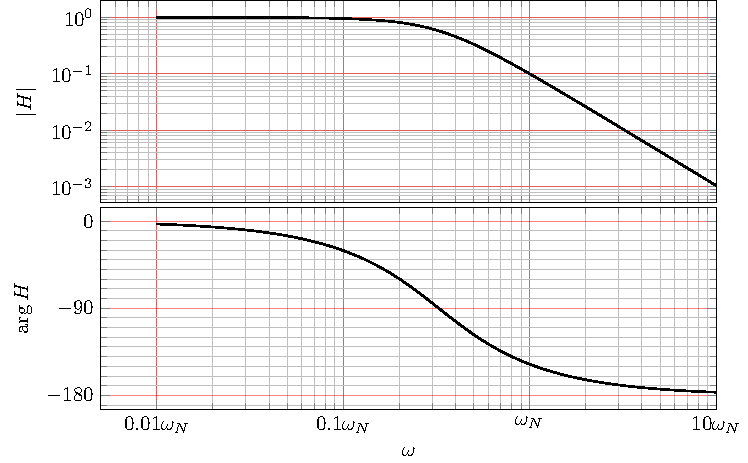
\includegraphics[width=0.8\linewidth]{../figures/ps7-bessel-bode}
\end{center}

\begin{enumerate}
\item What is the bandwidth of the filter?
\item Determine the filter parameter \(\omega_0\) in terms of \(\omega_N\).
\item What is the phase shift at the Nyquist frequency?
\item Assume that the cross-over frequency of the loop gain is \(\omega_c = 0.1\omega_N\). What is the phase shift at this frequency?
\item What delay $T$  does this correspond to? Approximate the filter as a pure delay \(H(i\omega) \approx \mexp{-i\omega T}\)?
\item How large is the delay in terms of the sampling period \(h = \frac{\pi}{\omega_N}\)?
\end{enumerate}


\section*{Choice of bandwidth of antialiasing filter}
\label{sec-2}

\begin{center}
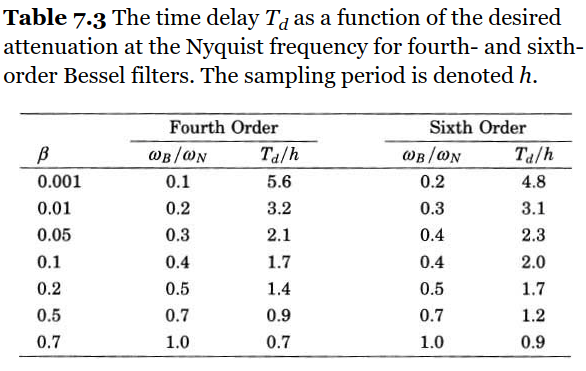
\includegraphics[width=0.4\linewidth]{../figures/Astrom-fig73.png}
\end{center}
The table can be used to find the delay incurred by an antialiasing filter. For instance, if we want to have an attenuation at the Nyquist frequency equal to \(\beta = 0.01\), then a fourth-order Bessel low-pass filter will give a delay of about \(T_d = 3.2 h\), that is a delay of more than 3 sampling periods. 
\begin{enumerate}
\item What is the advantage of using an antialiasing filter of higher order than 2?
\item If we can only accept a time delay of maximum two sampling periods, what is the attenutation we can obtain at the Nyquist frequency?
\item \(\omega_B = \omega_N\) means that the antialiasing filter is chosen so that the Nyquist frequency is the same as the bandwidth of the filter. The attenuation at \(\omega_N\) is then 0.7=-3dB. If the sampling period is 0.4 seconds. What is the time delay due to a sixth-order antialiasing filter?
\item What is the attenuation of a forth-order filter at \(5\omega_B\)
\end{enumerate}

\clearpage


\section*{Notch filter, preliminary exercise}
\label{sec-3}
Sketch the Bode diagram of the (unrealizable) filter
\[ F(s) = s^2 + \omega_1^2 = (s+i\omega_1)(s-i\omega_1)\]
\[ |F(i\omega)| = |(i\omega + i\omega_1)||(i\omega - i\omega_1)| = |\omega - (-\omega_1)||\omega - \omega_1|\]
\[ \arg F(i\omega) = \arg i(\omega + \omega_1) + \arg i(\omega -\omega_1) = 2\arg i + 0 + \arg(\omega - \omega_1) \]
\begin{center}
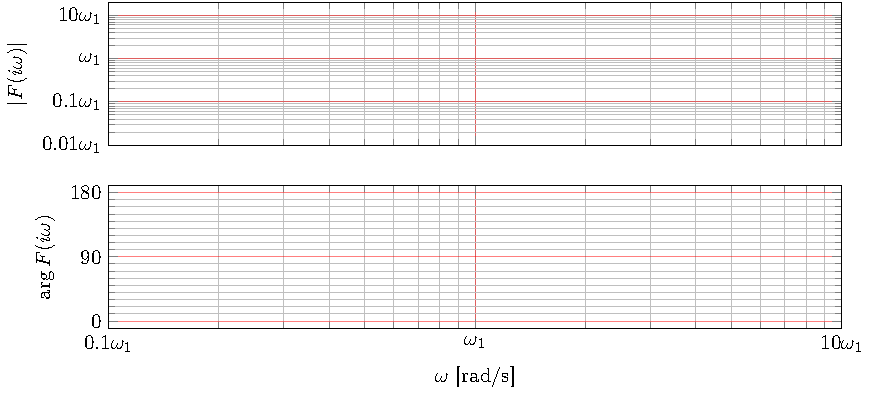
\includegraphics[width=0.85\linewidth]{../figures/bode-w1-empty}
\end{center}


\section*{Notch filter}
\label{sec-4}
Sketch the Bode diagram (\(Q=10\))of the second order continous-time notch filter
\[ F(s) = \frac{s^2 + \omega_1^2}{s^2 + \frac{\omega_1}{Q}s + \omega_1^2} \]

\begin{center}
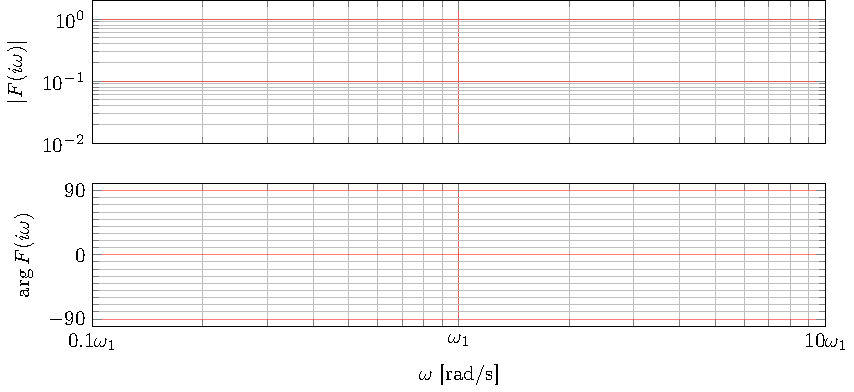
\includegraphics[width=0.85\linewidth]{../figures/bode-notch-empty}
\end{center}
% Emacs 24.5.1 (Org mode 8.2.10)
\end{document}